
%(BEGIN_QUESTION)
% Copyright 2005, Tony R. Kuphaldt, released under the Creative Commons Attribution License (v 1.0)
% This means you may do almost anything with this work of mine, so long as you give me proper credit

Studer denne trefase motorstyringskretsen (ofte kalt en ``bucket''), der sikringer beskytter mot overstrømsfeil, et trepolet relé (kalt en {\it kontaktor}) kobler kraften til og fra motoren, og et sett med overbelastningsvarmere registrerer moderate overstrømstilstander. Styringsledninger er utelatt for å forenkle. Bare kraftkoblingene er vist:

$$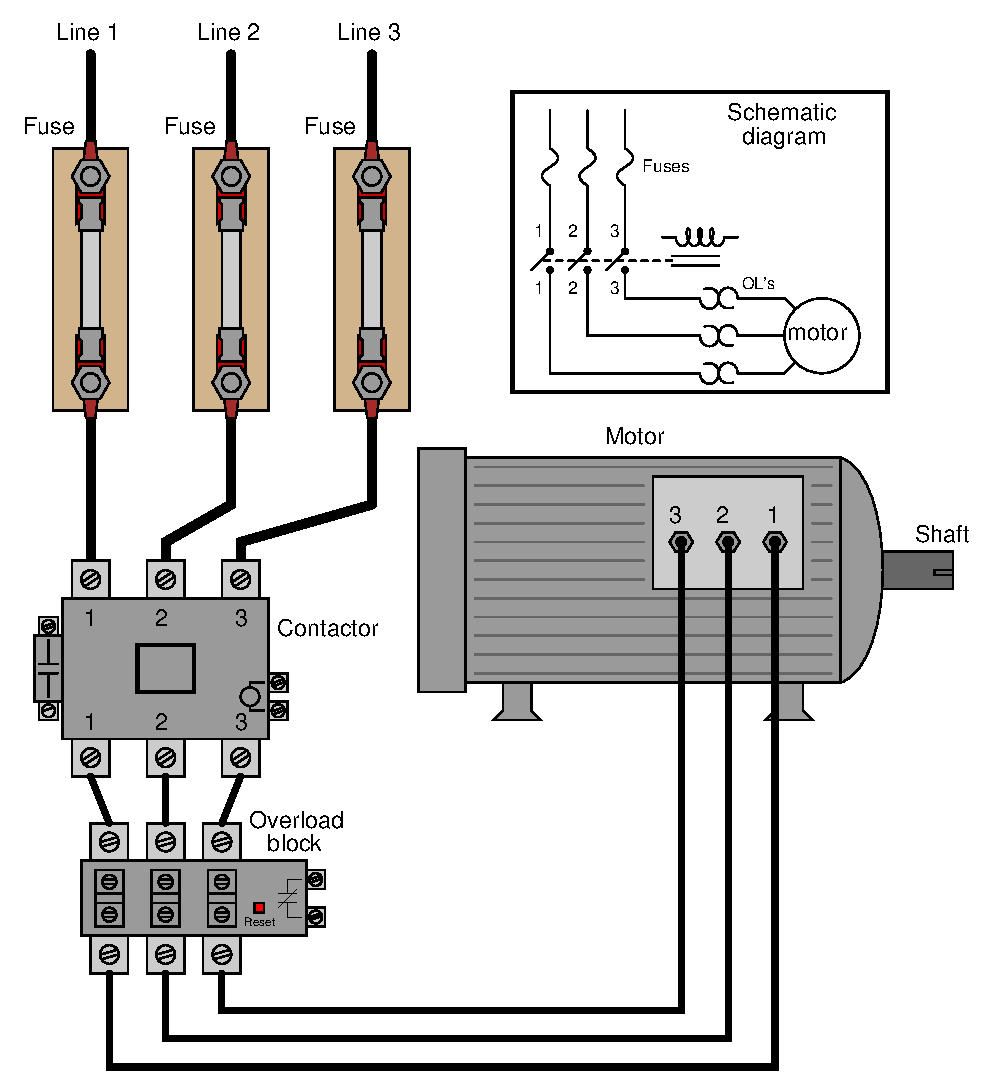
\includegraphics[width=15.5cm]{i01445x01.eps}$$

Etter mange års trofast drift nekter motoren en dag å starte. Den lager en ``summende'' lyd når kontaktoren energiseres (relékontaktene lukkes), men den roterer ikke. En mekaniker sjekker den og fastslår at akselen ikke har satt seg, men er fri til å rotere. Problemet må derfor være elektrisk!

Du blir tilkalt for å undersøke. Med et tangamperemeter måler du strømmen i hver av linjene (rett etter hver sikring) mens et nytt startforsøk gjøres. Deretter noterer du de tre strømmålingene:

% No blank lines allowed between lines of an \halign structure!
% I use comments (%) instead, so that TeX doesn't choke.

$$\vbox{\offinterlineskip
\halign{\strut
\vrule \quad\hfil # \ \hfil & 
\vrule \quad\hfil # \ \hfil \vrule \cr
\noalign{\hrule}
%
% First row
Linje & Strøm \cr
%
\noalign{\hrule}
%
% Another row
1 & 52.7 ampere \cr
%
\noalign{\hrule}
%
% Another row
2 & 51.9 ampere \cr
%
\noalign{\hrule}
%
% Another row
3 & 0 ampere \cr
%
\noalign{\hrule}
} % End of \halign 
}$$ % End of \vbox

Bestem minst to mulige feil, der hver av dem alene fullt ut kan forklare at motoren nekter å starte og de tre målte strømverdiene. Bestem deretter hva neste måling(er) skal være for å isolere nøyaktig plassering og natur på feilen.

\vskip 20pt \vbox{\hrule \hbox{\strut \vrule{} {\bf Forslag til sokratisk diskusjon} \vrule} \hrule}

\begin{itemize}
\item{} Finnes det en måte vi kunne avdekket mangel på strøm i linje 3 uten tangamperemeter, ved hjelp av et multimeter som ikke kan måle strøm direkte over 10 ampere?
\end{itemize}

\underbar{file i01445}
%(END_QUESTION)





%(BEGIN_ANSWER)

Her er noen muligheter:

\begin{itemize}
\item{} Sikring \#3 utløst (åpen)
\item{} Tredje relékontakt skadet (feilet åpen) inne i kontaktoren
\item{} Overbelastningsvarmer \#3 feilet åpen
\item{} Én vikling feilet åpen inne i motoren (forutsatt ``Y''-viklingskonfigurasjon)
\end{itemize}

Det finnes flere gyldige ``neste steg'' du kan ta herfra. Diskuter alternativer med medstudentene dine.

%(END_ANSWER)





%(BEGIN_NOTES)

At motoren summer men ikke roterer, sammen med totalt fravær av strøm i én linjeleder, forteller oss at motoren blir {\it enfaset}.

%INDEX% Electric motor (ORIGINAL GRAPHIC IMAGE FOR LIBRARY OBJECT)
%INDEX% Final Control Elements, motor: troubleshooting

%(END_NOTES)

